\documentclass{article}
\usepackage[utf8]{inputenc}
\usepackage{graphicx}
\graphicspath{{images/}}

\providecommand{\keywords}[1]
{
  \small	
  \textbf{\textit{Keywords---}} #1
}


\title{Automatic extraction of materials and properties from superconductors scientific literature}
\author{Authors}
% \date{March 2022}

\begin{document}

\maketitle

\begin{abstract}
The automatic extraction of materials and related properties from the scientific literature is getting more attention in data-driven materials science (Materials Informatics). 
We present our system for automatically extract superconductor material names and respective properties from PDF documents.
Our system combines Machine Learning and Heuristic approaches using a flexible architecture: developers can plug-in various Named Entities Recognition (NER) methods (CRF, BidLSTM, Transformers) or relation extraction approaches (ruled-based, CRF, Deep Learning).
We have processed X papers and extracted Y materials and properties: superconducting critical temperature, crystal structure and, when available, applied pressure and measurement method.
The data obtained is suitable as input in newly material discovery projects and is available in machine-readable format.
\end{abstract}

\keywords{material informatics, superconductors, machine learning, nlp, tdm}

\section{Introduction}

\section{Background and related work}
Introduction about the importance of structured data

Description of other work for creation of structured data 
 - CEDER 
 - J Callum tc and TC extraction from abstracts 


% Pedro/Terashima

Discussion on superconductors domain. Why superconductivity is still a la mode? What are the applications? Something along the same line of what we wrote in the SuperMat article. 

What are the current limits of SuperCon 1 from external users: data is fully manually inserted,no structure, the database contains more then 100 fields that were introduced freely 
Mistakes in SuperCon 1  

%Ishii-san?
Limits of Supercon 1 from internal perspective 
 - manually created 
 - users need to read the documents
 - expensive 
 - not easily extensible 
 
We can reference some examples of uses of Supercon1


\section{System}

We designed the system to follow the initial proposal \cite{foppiano:hal-02870896} which lay its foundations on the Grobid library for parsing and structuring scientific documents.
Reasons why we use the grobid library: 
 - exploit layout information
 - manage already pdf encoding crap 
 - plug-in machine learning architectures 
 - open source and maintained 
 
Describe in brief what we did and what the system does end to end. The next section will provide more details. 

\subsection{Architecture}


\begin{figure}[ht]
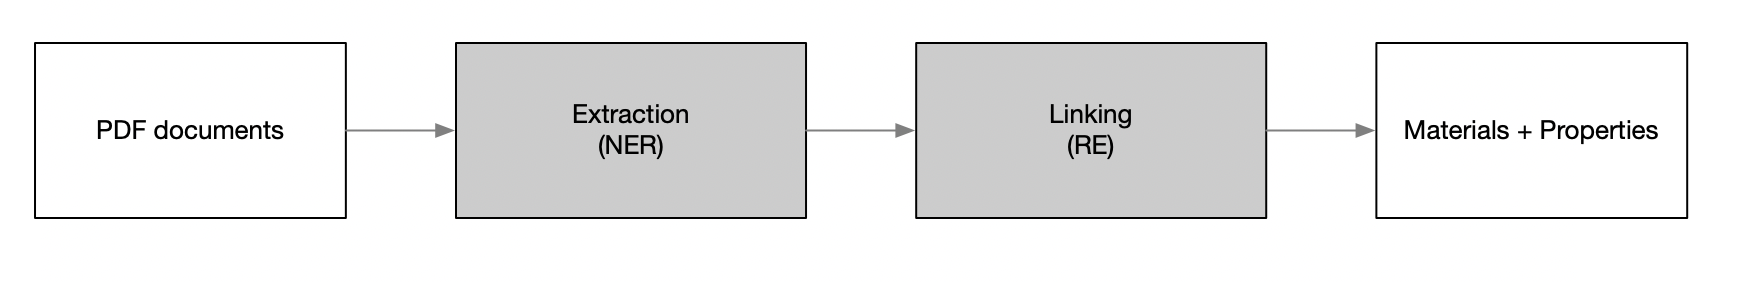
\includegraphics{overview-schema}
\caption{Overview of the architecture}
\end{figure}

\subsection{Extraction}

Description of the extraction 
 - models, features etc...
 
Evaluation

Table specifies what font sizes and styles must be used for each type of text in the manuscript.

\begin{table}[ht]
\centering
\begin{tabular}{lccc}
\hline \textbf{Label} & \textbf{Precision} & \textbf{Recall} & \textbf{F1-score} \\ \hline
class           & 79.69 & 75.54 & 77.55 \\
material        & 82.9  & 81.33 & 82.1  \\
me\_method       & 82.47 & 81.26 & 81.84 \\
pressure        & 65.03 & 54.01 & 58.26 \\
tc              & 84.63 & 80.73 & 82.63 \\
tcValue         & 79.3  & 74.95 & 76.97 \\
\hline
All (micro avg) & 82.43 & 79.68 & 81.03 \\
\hline
\end{tabular}
\caption{Evaluation scores of 10-fold cross-validation using the CRF architecture. }
\end{table}


\begin{table}[ht]
\centering
\begin{tabular}{lccc}
\hline \textbf{Label} & \textbf{Precision} & \textbf{Recall} & \textbf{F1-score} \\ \hline
class           & 81.84 & 83.96 & 82.85 \\
material        & 85.18 & 83.86 & 84.51 \\
me\_method      & 83.51 & 83.37 & 83.43 \\
pressure        & 63.79 & 73.24 & 67.98 \\
tc              & 83.70 & 81.66 & 82.66 \\
tcValue         & 73.23 & 80.73 & 76.76 \\
\hline
All (micro avg) & 83.01 & 82.89 & 82.95 \\
\hline
\end{tabular}
\caption{ Evaluation scores of 10-fold cross-validation using the RNN Bid-LSTM+CRF architecture. }
\end{table}

\begin{table}[ht]
\centering
\begin{tabular}{lccc}
\hline \textbf{Label} & \textbf{Precision} & \textbf{Recall} & \textbf{F1-score} \\ \hline
class           & 79.58 & 85.79 & 82.56 \\
material        & 83.89 & 86.13 & 84.99 \\
me\_method      & 83.92 & 86.50 & 85.19 \\
pressure        & 63.92 & 71.18 & 67.27 \\
tc              & 80.91 & 83.00 & 81.94 \\
tcValue         & 76.74 & 85.00 & 80.65 \\
\hline
All (micro avg) & 83.01 & 85.06 & 83.46 \\
\hline
\end{tabular}
\caption{Evaluation scores of 10-fold cross-validation using the Transformer architecture with SciBERT. }
\end{table}

Discussion of the results 

\subsection{Linking}

Introduction of the linking
Objective of the linking
Algorithm in brief (three or four different scenario): 
 - only one couple of entities 
 - multiple entities:
  - general amount: linking goes by distance 
  - respectively: linking goes in order 

Evaluation

\begin{table}[ht]
\centering
\begin{tabular}{lccc}
\hline \textbf{Linked entities} (Method) & \textbf{Precision} & \textbf{Recall} & \textbf{F1-score} \\ \hline
\textbf{material-tcValue} (Rule-based)  & 88.00 	&   74.00      &	81.00      \\
\textbf{material-tcValue} (CRF)         & 68.52 &	70.11   &  69.16    \\
\textbf{tcValue-pressure} (CRF) (CRF)   & 72.92 &	67.67   &  69.76    \\
\textbf{tcValue-me\_method} (CRF)       & 49.99 &	45.21   &  44.657   \\
\hline
\end{tabular}
\caption{Evaluation scores of the linking methods. }
\end{table}

Discussion on the linking, what works, what does not work 

\subsection{End to end evaluation}

What is the end 2 end evaluation? 
How the end 2 end evaluation is performed? 

Discussion of the results, which problems are currently emerging what are the prospective for the future?

\begin{table}[ht]
\centering
\begin{tabular}{lccc}
\hline \textbf{Precision} & \textbf{Recall} & \textbf{F1-score} & \textbf{Support} \\ \hline
73.86  &	66.33 &	69.90 & 597\\
\hline
\end{tabular}
\caption{End 2 end evaluation scores. }
\end{table}

\section{Supercon\textsuperscript{2}}

Introduction of the database, which data was extracted and the format 

\subsection{Ingestion workflow}

\begin{figure}[ht]
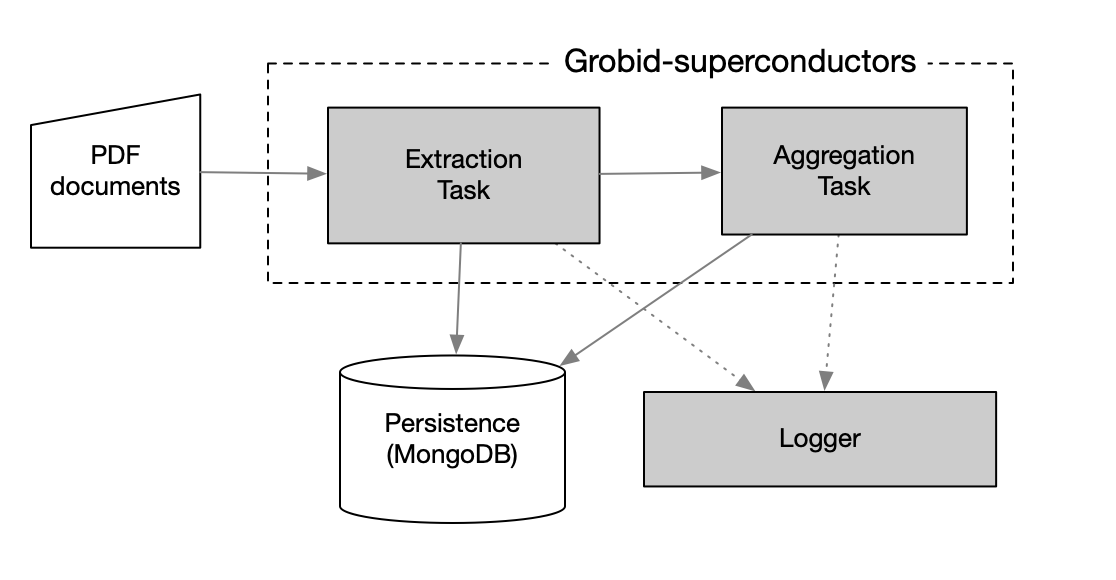
\includegraphics[width=\textwidth]{workflow-schema-1}
\caption{Schema of the ingestion workflow}
\end{figure}


Quickly discussion on the ingestion workflow 


\subsection{User interface}


\section{Conclusion}

\bibliography{bibliography}
\bibliographystyle{plain}


\end{document}
